\documentclass{article}
\title{Relazione 2: Generatori di numeri Pseudocasuali}
\author{Antonio Michele Miti}

\usepackage{amsmath}
\usepackage[utf8]{inputenc}
\usepackage[italian]{babel}
\usepackage{listings}
\usepackage{textcomp}
\usepackage{graphicx}
\usepackage{subfigure}
\usepackage{caption}
\usepackage{latexsym}
\usepackage{epstopdf}
\usepackage{eepic,epic,eepicemu}
\usepackage{color}
\pagestyle{headings}
\definecolor{listinggray}{gray}{0.9}
\definecolor{lbcolor}{rgb}{0.95,0.95,0.95}
\lstset{
	backgroundcolor=\color{lbcolor},
	rulecolor=,
	language=C++,
        basicstyle=\scriptsize,
        upquote=true,
        aboveskip={1.5\baselineskip},
        columns=fixed,
        showstringspaces=false,
        extendedchars=true,
        breaklines=true,
        prebreak = \raisebox{0ex}[0ex][0ex]{\ensuremath{\hookleftarrow}},
        frame=single,
        showtabs=false,
        showspaces=false,
        showstringspaces=false,
        identifierstyle=\ttfamily,
        keywordstyle=\color[rgb]{0,0,1},
        commentstyle=\color[rgb]{0.133,0.545,0.133},
        stringstyle=\color[rgb]{0.627,0.126,0.941},
}
\addtolength{\hoffset}{-1.25cm}
\addtolength{\voffset}{-1.80cm}
\addtolength{\textwidth}{1cm}
\addtolength{\textheight}{3.80cm}



\begin{document}
\maketitle
\begin{abstract}
Lo scopo di questo articolo è dare una soluzione numerica del problema matematico detto \emph{Ago di buffon}.
Dopo averne realizzato un modello computazionale si intende determinare una legge che descriva l'andamento dell'errore da attribuire ad una eventuale singola misura della \emph{probabilità di successo}.
Un'analisi teorica del problema porta ad individuare 3 fattori determinanti per stabilire una stima dell'incertezza della misura: errore sistematico, errore statistico, errore computazionale. Il primo errore origina della natura della legge che si intende calcolare sperimentalmente, ovvero la distribuzione di probabilità che è un'astrazione matematica definita esatta solo su infiniti lanci. 
L'errore statistico dipende dalla casualità delle singole variabili $ \left( \theta ,x \right) $ che determinano il successo del lancio. Infine l'errore computazionale è quello che emerge dalla non perfetta uniformità della distribuzione dei numeri generati dal generatore pseudocasuale \emph{rand} delle librerie \emph{C++}.
\end{abstract}
%\tableofcontents


\section{Introduzione}
\paragraph{Il problema dell Ago di Buffon :}

Si consideri un pavimento, suddiviso da un grande numero di righe paralle equispaziate da una distanza \emph{T}, si immagini ora di lasciar cadere su di esso, in modo completamente casuale, un sottile ago di lunghezza \emph{R}. Scopo del problema è determinare con quale probabilità l'ago, una volta caduto, si trovi a contatto con almeno una delle righe sul piano. 

\subsection{Analisi Teorica}
In termini matematici i gradi di libertà che descrivono il sistema sono solo 2: le variabili $(\theta,x)$ che fissano la posizione del ago sul piano. 
La variabile $ \theta $ fissa l'inclinzione dell ago rispetto alle righe parallele, mentre la variabile $x$ esprime la distanza del centro di massa dell ago dalla riga più vicina.

	\begin{figure}[htbp]
	\centering
	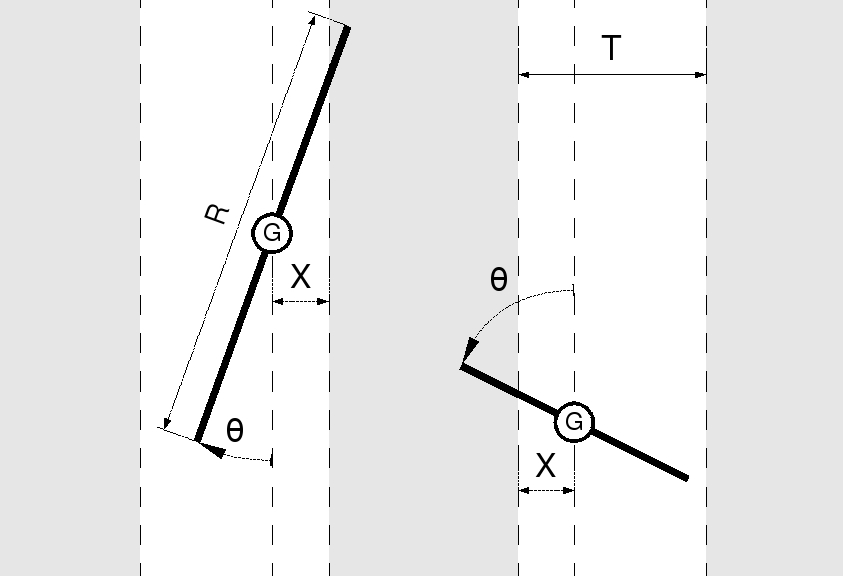
\includegraphics[height=6cm,,keepaspectratio]{disegno.jpg}
	\caption{Parametri dell ago di buffon}
	\end{figure}

Un lancio è considerato un successo quando l'ago, una volta fermo sul piano, tocca almeno una riga parallela. Da semplici considerazioni geometriche si ottiene che la condizione di successo è :

	\begin{equation}
	\textrm{condizione di successo :}\qquad x \leq \frac{R}{2}\sin(\theta)
	\end{equation}
%$$ x \leq R\sin(\theta) $$

Considerando la caduta del ago come un evento perfettamente casuale le coordinate di configurazione del sistema possono assumere equiprobabilmente qualsiasi valore compreso negli intervalli

	\begin{equation}
	0 \leq x \leq \frac{T}{2}\qquad
	\textrm{e}\qquad
	0 \leq \theta \leq \frac{\pi}{2}
	\end{equation}

Più precisamente questa condizione equivale ad affermare che $ \left( \theta ,x \right) $ sono una coppia di variabili aleatorie con funzione densità di probabilità uniforme.
Ciò significa che le funzioni densità di probabilità delle 2 variabili dovranno essere delle costanti che intragrate sugli intervalli (2) diano la probabilità totale 1.
$$ 1=\int_{R}f(t)dt=k\int_{I}dt=K(x1-x0)\qquad\Longrightarrow$$ 
	\begin{displaymath}
	g(\theta)=\dfrac{2}{\pi}
	\qquad
	h(x)=\dfrac{2}{T}
	\end{displaymath}

L'indipendenza delle due variabile aleatorie permette di fattorizzare la funzione densità di probabilità $f(\theta,x)$ come il prodotto delle due singole funzioni.
 	\begin{equation}
	f(\theta,x)=g(\theta)h(x)=\dfrac{4}{T\pi}
	\end{equation}
A questo punto è sufficiente integrare la funzione densità di probabilità sul dominio $D$, in cui le variabili aleatorie danno un successo, per ottenerè la probabilità che l'ago tocchi almeno una riga sul pavimento.
 	\begin{equation}
	P_{successo}=\int_{0}^{\frac{\pi}{2}}\int_{0}^{\frac{R}{2}\sin(\theta)}\dfrac{4}{T\pi}dxd\theta 
	=\dfrac{2R}{T\pi}
	\end{equation}

\subsection{Simulazione del esperimento in C++}

Il modello per la simulazione è molto semplice: si usa la funzione rand() delle librerie C++ per estrarre 2 numeri casuali negli intervalli (2), se la coppia di valori soddisfa la condizione (1) asi ha un successo.

Ripetendo la simulazione di un lancio un numero $N$ di volte e ottenendo complessivamente un numero $k$ di successi, si ottiene una stima della probabilità di successo:
	\begin{equation}
	P_{successo}(N)=\dfrac{k}{N}
	\end{equation}
Risulta la seguente funzione di C++;

\begin{lstlisting}[frame=single]
int cont=0; //contatore delle volte che l'ago tocca una fessura
for(int i=0; i<N; i++)	{ 
	double x = ((double)rand()/RAND_MAX)*T/2;
	double s = ((double)rand()/RAND_MAX)*(M_PI/2);
	if(x<=(R/2)*sin(s))cont++ ;} // condizione di successo
return probabilita=((double)cont/N); 
\end{lstlisting}

A questo punto bisogna stabilire con che incertezza un singolo \emph{esperimento} di N lanci determina la stima della probabilità di successo, si cerca una leggi in funzione del numero dei lanci componenti l'esperimento.

\subsection{Errore sistematico}

Il concetto di probabilità relativo ad un particolare evento può essere definito come limite  di (5) per un numero $N$ di prove tendente all'infinito.

Qualsiasi simulazione computazionale o esperimento empirico invece prevede necessariamente un numero finito di prove, di fatto può solo stimare, con una certa approssimazione, il valore della probabilità.

Considerando una simulazione di $N$ lanci, la casualità delle variabili aleatorie implica che anche il numero $k$ di successi sia casuale (ovviamente con una distribuzione diversa, cambierà ogni volta che si ritenta la simulazione [vedere errore statistico]) e potrà in generale assumere ogni valore intero compreso tra $0$ e$K$ .
Quindi se :

	\begin{displaymath}
	P=\dfrac{k}{N}
	\qquad e \qquad
	P'=\dfrac{k\pm1}{N}
	\end{displaymath}

i vari valori di $P$ risultanti dall'esperimento non potranno assumere valori continui ma tutti i possibili risultati saranno distanziati da un intervallo:

	\begin{displaymath}
	\bigtriangleup P = \mid P-P' \mid = \dfrac{1}{N} .
	\end{displaymath}

Dato che il valore atteso di $P$ è un numero irrazionale (contiene $\pi$) sarà necessariamento compreso tra una certa coppia di valori $(P , P')$ che invece, in quanto quozienti di numeri naturali, risulteranno sempre una quantità razionale. 

	\begin{figure}[htbp]
	\centering
	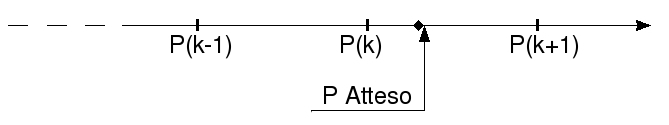
\includegraphics[width=10cm,keepaspectratio]{disegno2.jpg}
	\caption{Errore sistematico: con P(K) si intende la probabilità risultante da k successi.}
	\end{figure}

Per cui il valore di $P$ risultante da una simulazione di $N$ prove approssima la probabilità vera con un incertezza:

	\begin{equation}
	\delta_{sistematico}=\dfrac{\bigtriangleup P}{N}=\dfrac{1}{2N}	.
	\end{equation}

\subsection{Errore statistico}

Come accennato nella sezione precedente, la casualità delle variabili aleatorie implica che anche il numero $k$ di successi sia casuale. In linea di principio ogni simulazione darà un risultato di $P$ leggermente diversa da quello precedente con una distribuzione gaussiana attorno al valore atteso.

\begin{figure}[htbp]
	\centering
	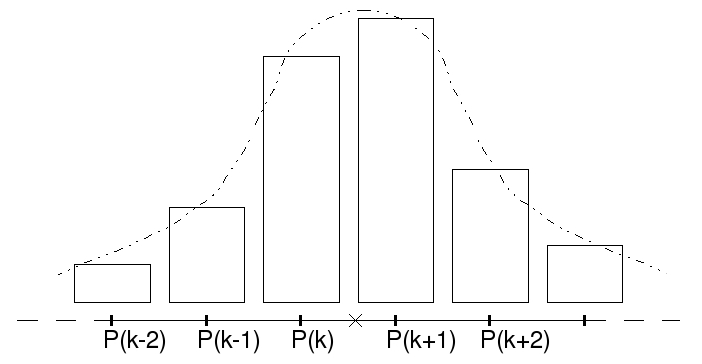
\includegraphics[width=10cm,keepaspectratio]{disegno3.jpg}
	\caption{Andamento atteso a causa dell'errore statistico.}
	\end{figure}

L'errore statistico sarà dunque la \emph{deviazione standard} del risultato di $K$ simulazioni da $N$ lanci ciascuna:

	\begin{equation}
	\delta_{statistico}=\sqrt{\mid \bar{x^{2}}-\bar{x}^{2}\mid}= ...
	\end{equation}

A questo punto si sarebbe tentati ad utilizzare la media dei risultati degli esperimenti come stima di P, questo è chiaramente sensato ma computazionalmente è identico ad un singolo esperimento di $K$ x $N$ lanci:

	\begin{equation}
	\bar{P}=\dfrac{\sum_{i=1}^{K}\dfrac{successi_{i}}{N}}	{K}=\dfrac{\sum_{i=1}^{K}successi_{i}}{NK}
	\end{equation}

In sostanza questo errore esprime, nell'ipotesi di uniformità della funzione di probabilità del generatore rand(), la dispersione del valore ottenuto attorno al valore vero per colpa della casualità dei possibili risultati di un singola simulazione di esperimento.

\subsection{Errore computazionale}

Questo errore deriva dalla pseudo-casualità del generatore.

Non ci sono motivi di dubitare dell'efficienza della funzione rand() di \emph{C++}, che è già stata immensemente testata, ma in ogni caso ogni algoritmo numerico presenta dei difetti: crea catene di valori interi, periodiche, finite, numerabili; sono deterministici: partendo da un seed si avrà ogni volta la stessa catena; nel complesso possono solo \emph{approssimare} una distribuzione uniforme su un intervallo continuo...

Nello specifico non è possibile fare una stima a priori dell'incertezza causata da questi fattori, il solo concetto di "casuale" è problematico da definire per una catena finita di valori.

Questo però non impedisce di fare una stima di questa incertezza.
Inanzi tutto è evidente che il generatore pseudo-random entra solo nel momento in cui la simulazione chiama una coppia di valori $ \left( \theta ,x \right) $, l'imperfezione del generatore implicherà che le distribuzioni di probabilità relative ai 2 parametri siano solo "quasi" uniformi, ovvero esisteranno  due funzioni $(\eta(\theta),\upsilon(x))$ tali per cui le effettive funzioni densità di probabilità per le 2 variabili saranno:

	\begin{displaymath}
	g(\theta)=\dfrac{2}{\pi}(1+\eta(\theta))
	\qquad
	h(x)=\dfrac{2}{T}(1+\upsilon(x))
	\end{displaymath}

la forma delle funzioni dipenderà dal tipo di generatore mentre il loro modulo sarà legato all'efficienza.
A questo punto si potrebbe sfruttare l'indipendenza delle 2 variabili aleatorie e costruire la funzione  densità di probabilità totale, il punto è che chiamando successivamente 2 rand() non si fa altro che prendere un elemento e il suo successivo nella stessa catena, data la natura "linear congruent math" del algoritmo l'indipendenza delle due variabili aleatorie non è garantita.

La conseguenza di tutto questo si esprimerà con una funzione di correzione $\varepsilon*W(\theta,x)$ alla funzione distribuzione di probabilità del problema.
In altre parole la distribuzione di probabilità vera risulta:

	\begin{equation}
	f(\theta,x)=\dfrac{4}{T\pi}(1+\varepsilon W(\theta,x))
	\end{equation}

Per cui la probabilità di avere un successo in questo modello imperfetto sarà:
	\begin{equation}
	P_{successo}^{simulazione}=\int_{0}^{\frac{\pi}{2}}d\theta\int_{0}^{\frac{R}{2}\sin(\theta)}\dfrac{4}{T\pi}(1+\varepsilon W(\theta,x))dx
	=P_{successo}^{teorico} - \varepsilon\int\int W(\theta,x)d\theta dx
	\end{equation}
quindi si arriva ad una stima del errore random:
	\begin{equation}	
	\delta_{random}=\mid P_{successo}^{teorico} - P_{successo}^{simulazione} \mid \approx \varepsilon
	\end{equation}
che evidentemente non dovrebbe dipendere dal numero $N$ di lanci della simulazione. 

\section{Metodologia}
Scopo della relazione è dare una stima dell'incertezza sul risultato della simulazione in funzione del numero di lanci di ciascuna simulazione.
\paragraph{Errore Sistematico :}
L'andamendo dell'errore sistematico è noto a priori $\dfrac{1}{2N}$.

\paragraph{Errore Statistico :}
Vengono simulati, al variare del parametro $N$= numero dei lanci,  100 esperimenti di Ago di Buffon generando un insieme $\{ P_{i} \}$ di 100 risultati in funzione di N.
Per ogni set viene calcolata la media e la deviazione standard allo scopo di mostrare graficamente l'andamento dell'errore in funzione di N e di eseguirne un fit tramite gnuplot in modo da ricavare la legge cercata.

\paragraph{Errore Computazionale :}
Si esegue un'altra analisi sul set di valori ottenuti prima stampando l'andamento del modulo della differenza P(n)-P(atteso) in funzione del numero di lanci fatti nel esperimento.

Sapendo che teoricamente vale:
$$ lim_{n \to \infty}P^{sperimentale}(n)=P^{teorico}$$
fittando i dati considerati con una funzione con parametro libero costante del tipo
$$f(n)= A+g(n,B,C,D...)$$
dove $(A,B,C,D..)$ sono i parametri liberi del fit e $g(n)$ è una funzione evanescente a $+\infty$, il parametro A sarà la stima dell'errore computazionale causato dal generatore.




\clearpage
\section{Risultati}
\paragraph{Errore statistico}
Per evedenziare l'effetto del errore statistico è possibile costruire un istogramma [\figurename \ref{fig:isto}] che conti il risultato di un certo numero di simulazioni da 10 lanci.
\begin{figure}[htbp]
	\centering
	\caption{Istogramma della dispersione, dal valore atteso, dei risultati di K simulazioni da 10 lanci ciascuna. }	%Output di dubbioni2.c
	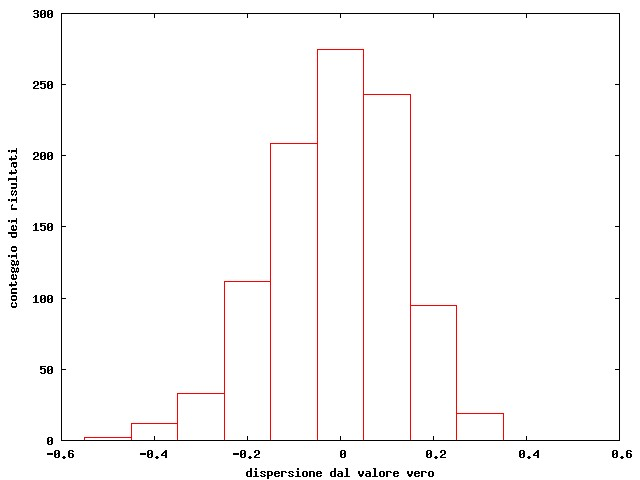
\includegraphics[height=8cm,,keepaspectratio]{dispersione.jpg}
	\label{fig:isto}
	\end{figure}
Come si vede dal grafico la distribuzione dei risultati è piccata attorno al valore vero ma presenta in ogni caso una certa dispersione sui valori.
Per questo è necessario prendere la media di questi valori per ottenere una stima accettabile della probabilità cercato.

Simulando, al variare del parametro $N$= numero dei lanci,  100 esperimenti di Ago di Buffon è possibile costruire il grafico della stima della probabilità in funzione del numero dei lanci :[\figurename \ref{fig:ago1}].
	\begin{figure}[htbp]
	\centering
	\caption{Grafico del andamento del valore medio di $P(n)$ con rappresentato la somma degli errori statistico e sistematico in funzione del numero dei lanci. Output di ago\_1.c}
	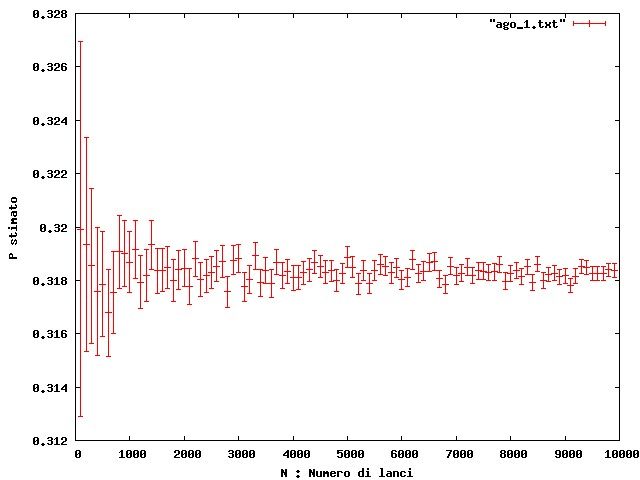
\includegraphics[width=13cm,,keepaspectratio]{ago_1.jpg}
	\label{fig:ago1}
	\end{figure}

L'errore rappresentato è l'effetto complessivo degli errori statitistici e sistematici quindi il grafico converge al valore $P_{stimato}^{simulazione}$.

Inoltre è possibile dare una stima dell'errore statistico stampando la deviazione standard di 100 esperimenti al variare di $N$, numero dei lanci:[\figurename \ref{fig:ago2}].

	\begin{figure}[htbp]
	\centering
	\caption{Grafico del andamento della deviazione standard sulla media di $P(n)$ in funzione del numero dei 	lanci} %. Output di ago\_2.c.
	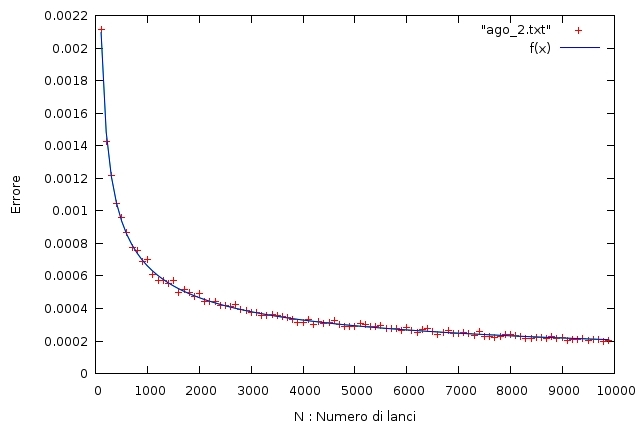
\includegraphics[width=13cm,keepaspectratio]{ago_2.jpg}
	\label{fig:ago2}
	\end{figure}

A questo punto è possibile fare un fit dei valori, ci si aspetta un andamento del tipo:
	\begin{equation}
	\delta_{statistico} (N)=AN^{B}
	\end{equation}
quindi fittando, tramite gnuplot, secondo la funzione \emph{ f(x) =A\*x\*\*B}, si ottiene il seguente output:

\begin{lstlisting}[frame=single]
After 265 iterations the fit converged.
final sum of squares of residuals : 1.57567e-08
rel. change during last iteration : -3.2102e-08

degrees of freedom    (FIT_NDF)                        : 97
rms of residuals      (FIT_STDFIT) = sqrt(WSSR/ndf)    : 1.27452e-05
variance of residuals (reduced chisquare) = WSSR/ndf   : 1.6244e-10

Final set of parameters            Asymptotic Standard Error
=======================            ==========================

A               = 0.0211063        +/- 0.0002628    (1.245%)
B               = -0.501652        +/- 0.001838     (0.3664%)
\end{lstlisting}

In conclusione l'andamento di $\delta_{statistico} (N)$ è del tipo:
$$	\delta_{statistico} (N)\sim\frac{1}{\sqrt{N}}$$

\paragraph{Errore computazionale}
Per stimare l'errore computazionale è necessario studiare la convergenza della simulazione.
Quindi si stampa il valore assoluto della differenza tra valore atteso $\frac{2R}{T\pi}$ e la media di 1000 simulazioni, ottenendo il grafico :[\figurename \ref{fig:ago2}].
	\begin{figure}[h]
	\centering
	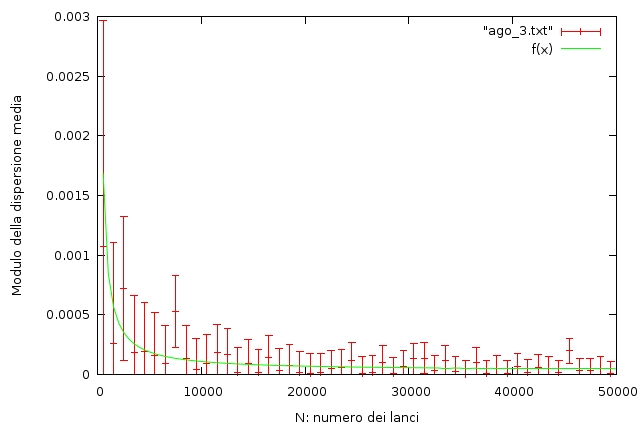
\includegraphics[width=10cm,,keepaspectratio]{ago_3.jpg}
	\caption{Grafico del andamento del modulo della dispersione della media rispetto al valore atteso in funzione dei lanci considerando gli errori precedentemente stimati.}
		\label{fig:ago3}
	\end{figure}

A questo punto è possibile fittare i dati trovati con una funzione del tipo:
	\begin{equation}
	f(N)=A+N^{B}
	\end{equation}
il parametro A restituirà una stima dell'incertezza derivante dal \emph{errore computazionale} mentra il parametro B indicherà la convergenza del modello al valore atteso.

\begin{lstlisting}[frame=single]
After 46 iterations the fit converged.
final sum of squares of residuals : 8.30531
rel. change during last iteration : -7.1159e-07

degrees of freedom    (FIT_NDF)                        : 48
rms of residuals      (FIT_STDFIT) = sqrt(WSSR/ndf)    : 0.415965
variance of residuals (reduced chisquare) = WSSR/ndf   : 0.173027

Final set of parameters            Asymptotic Standard Error
=======================            ==========================

A               = 3.37606e-05      +/- 1.319e-05    (39.08%)
B               = -1.02927         +/- 0.03679      (3.574%)
\end{lstlisting}

Risulta che il modello converge al valore atteso come $1/N$ mentre
	\begin{equation}
	\delta_{computazionale}\simeq 4 \times 10^{-5}
	\end{equation}

\clearpage
%\section{Case-Study}
\section{Conclusione}
Si ottengono le seguenti leggi per l'errore:
\begin{center}
\begin{tabular}{|c|c|}
\hline
 & \\$\delta_{sistematico}$ & $\sim \dfrac{1}{2N}$ \\ & \\
\hline
 & \\$\delta_{statistico}$ & $\sim 0,02\dfrac{1}{\sqrt{N}}$ \\ & \\
\hline
 & \\$\delta_{computazionale}$ & $\sim 4 \times 10^{-5}$\\ & \\
\hline
\end{tabular}
\end{center}
Mettendole a confronto si nota che per simulazioni con pochi lanci domina su tutti l'errore sistematico, la situazione si inverte superando i 500 lanci da dove comincia a dominare l'errore statistico.
Per la totalità dei casi pratici l'incertezza computazionale risulterà completamente trascurabile rispetto alle altre fonti di errore.


	\begin{figure}[h]
	\centering
	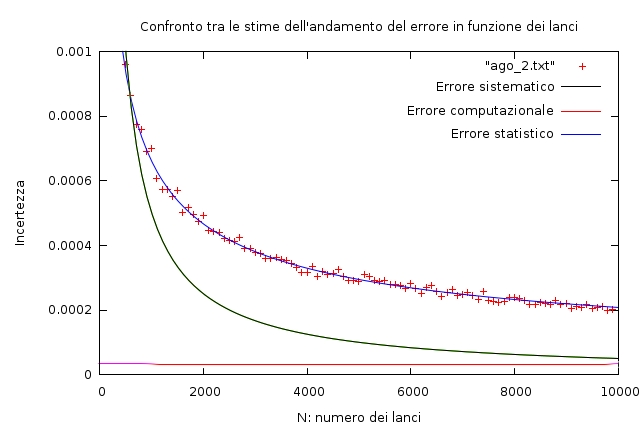
\includegraphics[width=10cm,,keepaspectratio]{confronto.jpg}
	\end{figure}


\clearpage
\begin{thebibliography}{99}
\bibitem{recipe}\emph{Numerical recipes in C++}
\bibitem{knuth}Knuth D. \emph{The Art of Computer Programming}
\bibitem{hilde}Hildebrand F. \emph{Introduction to Numerical Analysis}, 2nd.ed.
\end{thebibliography}
\end{document}
